\chapter{Appendix}

\begin{figure}[!ht]
    \centering
    \subfloat[Amplitude \(\hat{U}\)\label{subfig:pulsAmplitude}]{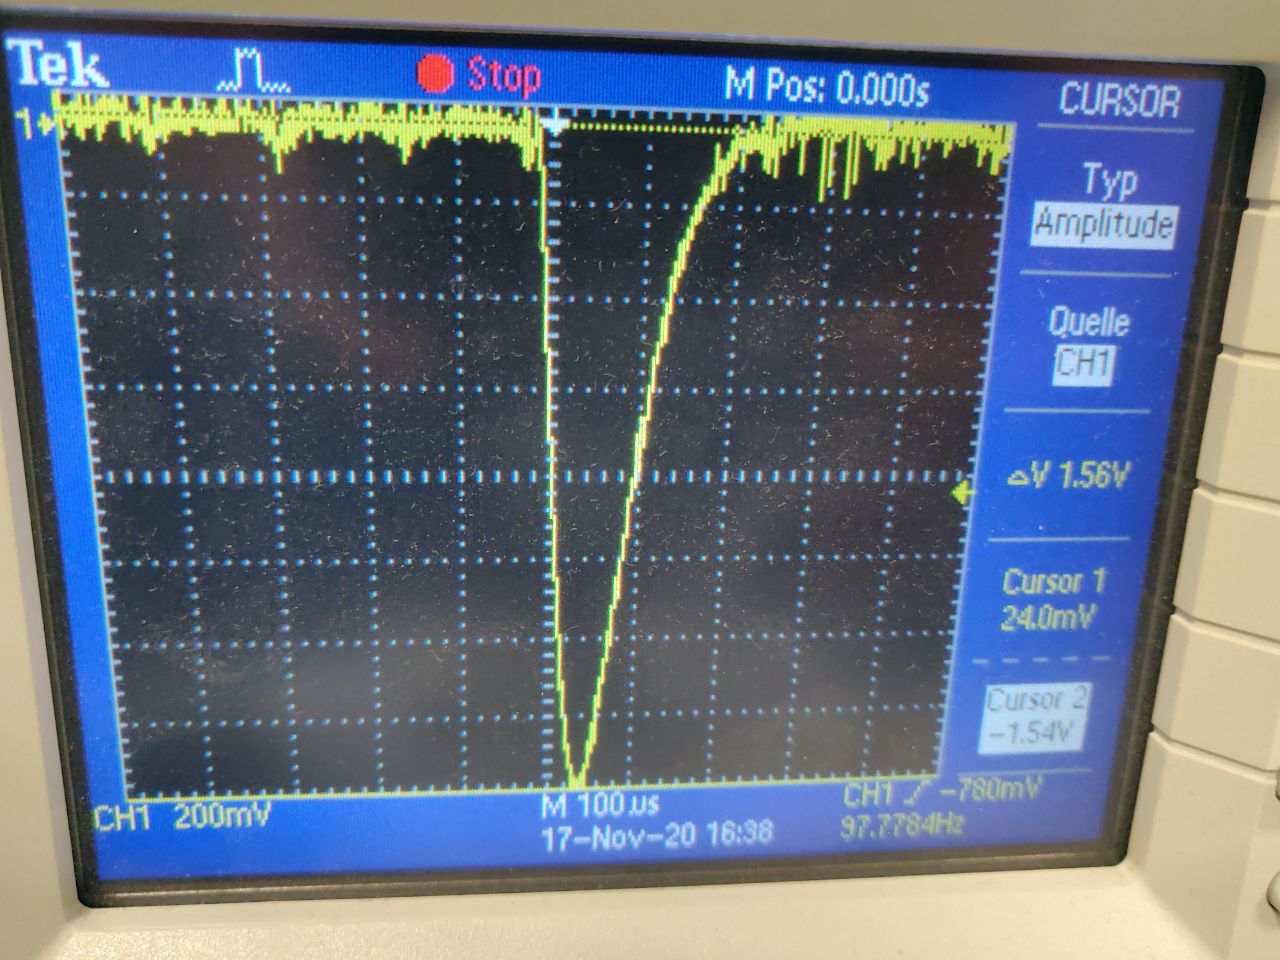
\includegraphics[width=0.45\textwidth]{messdaten/Fig.1_pulsAmplitude.jpg}}
    \hspace{.05\textwidth}
    \subfloat[Fall Time \(t_{f}\)\label{subfig:fallTime}]{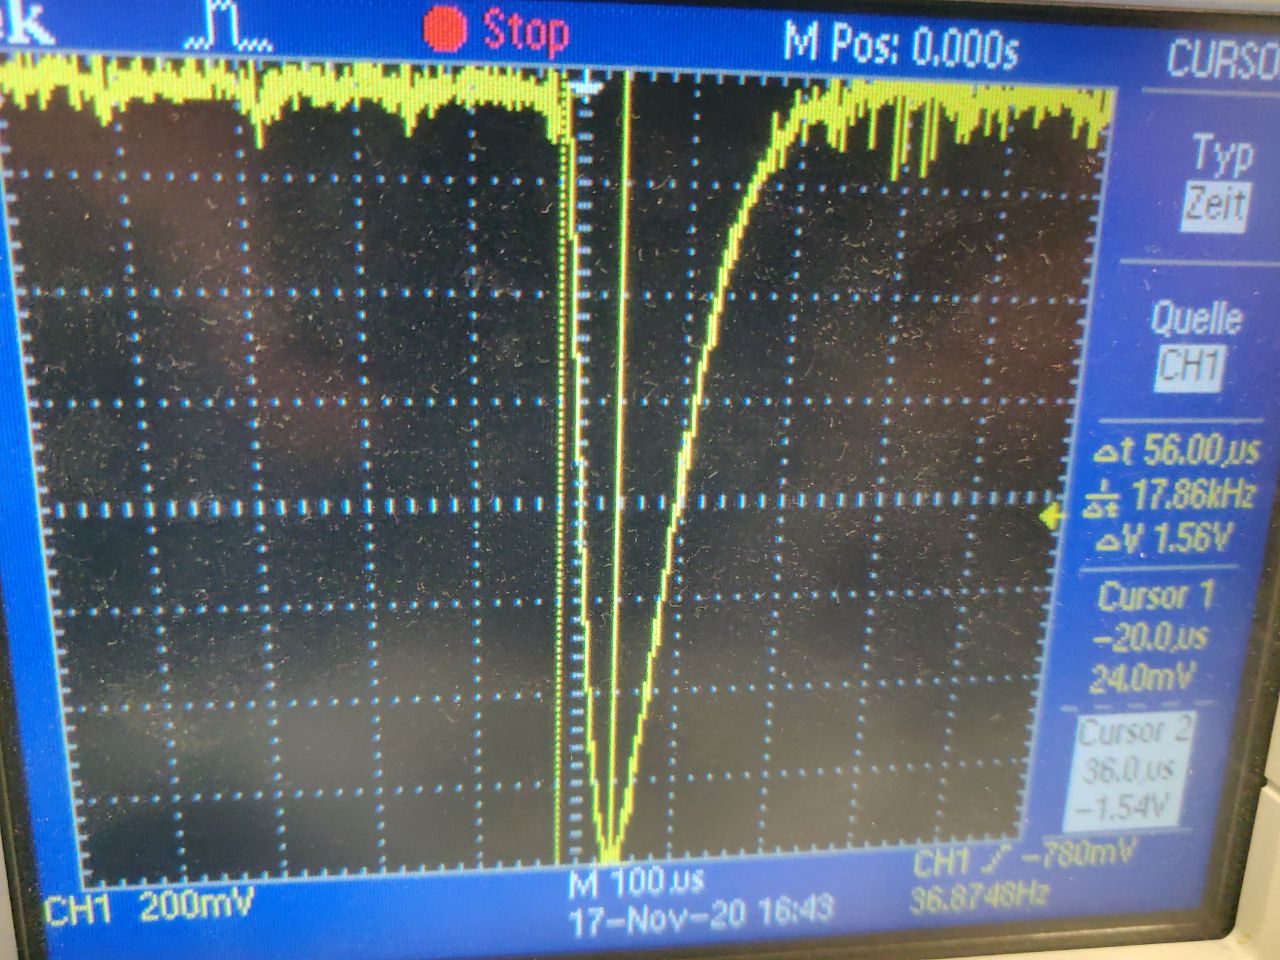
\includegraphics[width=0.45\textwidth]{messdaten/Fig.2_fallTime.jpg}}
    \hspace{.2\textwidth}
    \subfloat[Rise Time \(t_{r}\)\label{subfig:riseTime}]{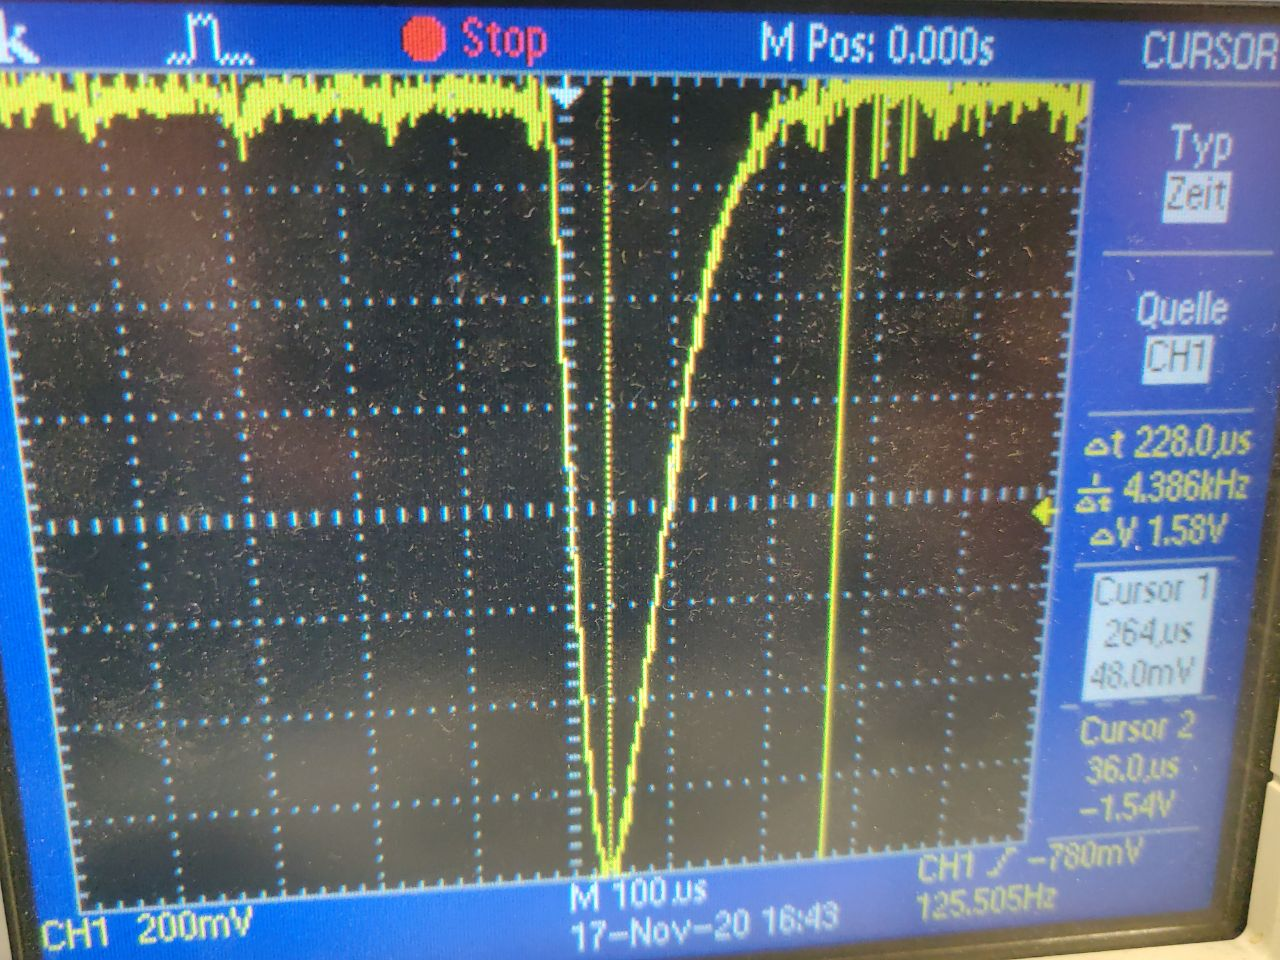
\includegraphics[width=0.45\textwidth]{messdaten/Fig.3_riseTime.jpg}}
    \hspace{.05\textwidth}
    \subfloat[Pulse Width \(t_p\)\label{subfig:pulseWidth}]{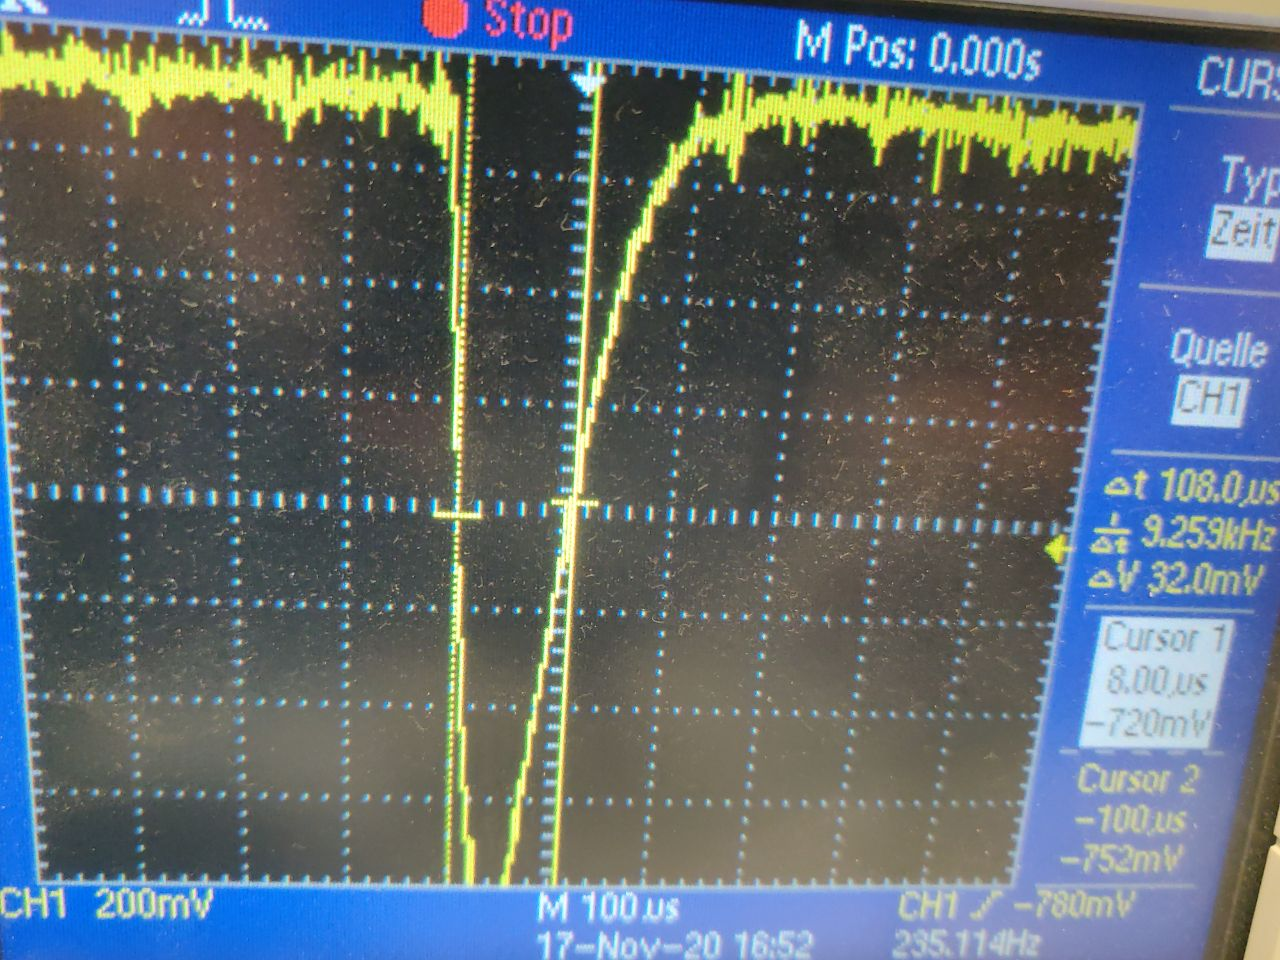
\includegraphics[width=0.45\textwidth]{messdaten/Fig.4_pulseWidth.jpg}}
    \hspace{.2\textwidth}
    \subfloat[Recovery Time \(t_{r}\)\label{subfig:recoveryTime}]{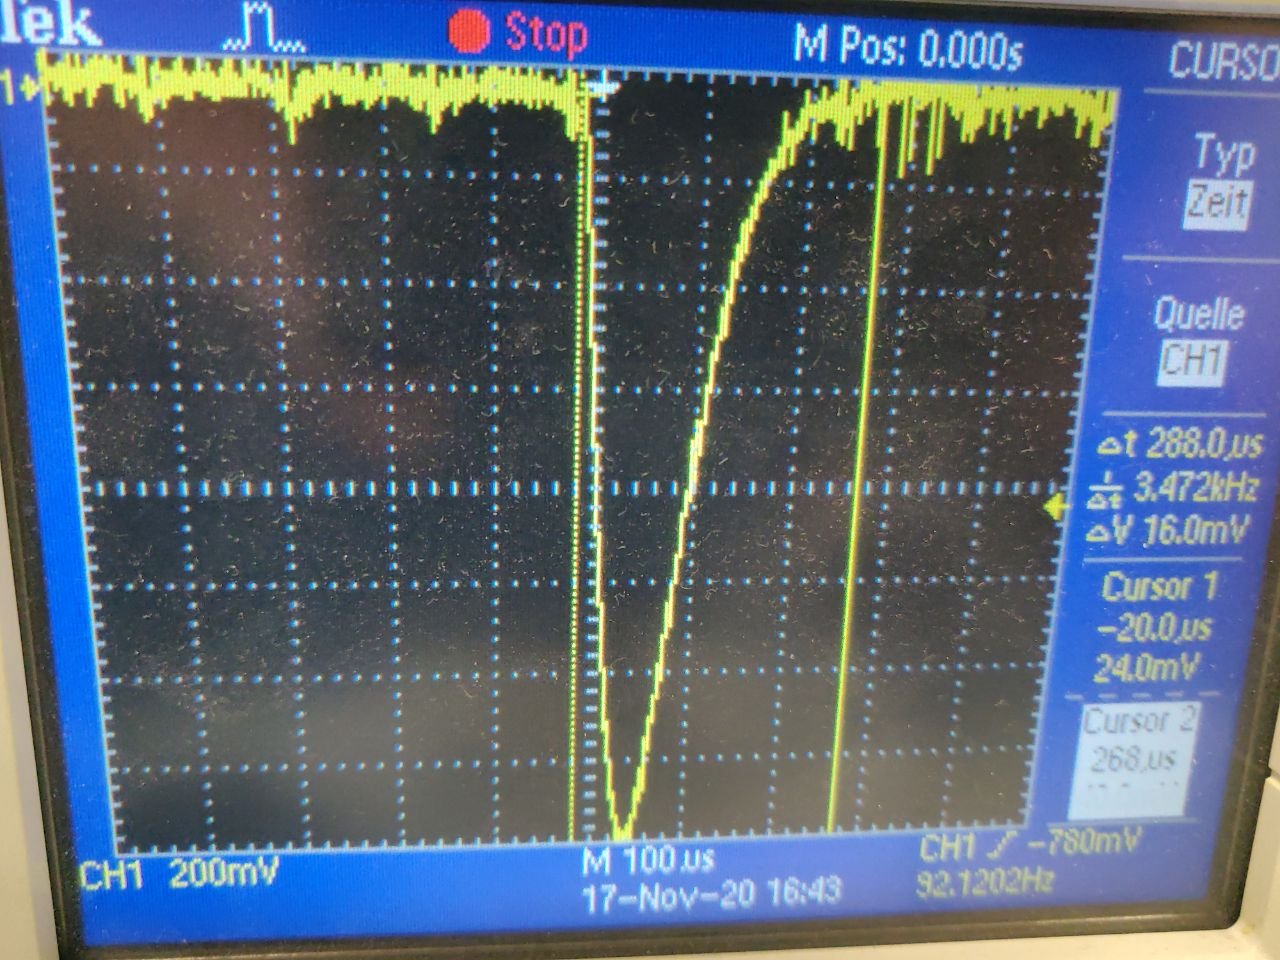
\includegraphics[width=0.45\textwidth]{messdaten/Fig.5_recoveryTime.jpg}}
    \caption[Oszillograms]{During the course of the experiment captured oscillograms.}
 \end{figure}
 %
 \newpage
 %